%%%% Proceedings format for most of ACM conferences (with the exceptions listed below) and all ICPS volumes.
\documentclass[sigconf]{acmart}
\usepackage{tikz}

\begin{document}

\title{Community Detection on Higher-Order Networks: Identifying Patterns in U.S. Air Traffic}

% The "author" command and its associated commands are used to define the authors and their affiliations.
\author{Bradley Dice}
\email{bdice@bradleydice.com}
\orcid{0000-0002-9983-0770}
\affiliation{
  \institution{University of Michigan \\ Department of Physics}
  \city{Ann Arbor}
  \state{Michigan}
  \postcode{48109}
}

\author{Daniel McCusker}
\email{dmccuske@umich.edu}
\affiliation{
  \institution{University of Michigan \\ Applied Physics}
  \city{Ann Arbor}
  \state{Michigan}
  \postcode{48109}
}

\author{Shannon Moran}
\email{moranse@umich.edu}
\orcid{0000-0002-3579-3149}
\affiliation{
 \institution{University of Michigan \\ Department of Chemical Engineering}
  \city{Ann Arbor}
  \state{Michigan}
  \postcode{48109}
 }

\renewcommand{\shortauthors}{Dice, et al.}
\settopmatter{printfolios=true} % puts in page numbers

% The abstract is a short summary of the work to be presented in the article.
\begin{abstract}
In this project, we studied the utility of higher-order network (HON) representations for trajectory data. For our trajectory data, we used publicly available airline ticket data sets which have previously been used as a model system in the literature \cite{Rosvall2014}. Here, we demonstrate that variable-order HONs can be built from this data. Further, we demonstrate that a random-walker-based community detection method ``InfoMap,'' previously used on shipping data, is able to successfully find meaningful communities on the HON. We are able to validate these communities by comparing them to known airline traffic structures, mapping communities onto local networks primarily served by one carrier. Finally, we show that these community structures are largely maintained even after airlines merge---indicating that while airline mergers impact the business of airlines (ticket names, scale, etc.), they leave the underlying traffic structure largely untouched. We conclude that variable order HONs are indeed able to identify meaningful structure in air traffic transportation networks.
\end{abstract}

% Show author, affiliation, and title information
\maketitle

% \section{Guidelines}
% Length: 8 pages including citations. If a section is not listed here, Shannon considers it done-- feel free to make edits.
% \begin{itemize}
%     % \item Section 1. Abstract - DONE
%     % \item Section 2. Introduction - Shannon to do
%     % \item Section 3. Data - DONE
%     \item Section 4. Methods - needed parts highlighted in color
%     \item Section 5. Experiments - needed parts are highlighted in color
%     \item Section 6. Related Work - two paragraphs needed (one a nice-to-have), highlighted in color
%     % \item Section 7. Conclusions - DONE
%     % \item Section 8. Division of work - DONE, plz review
% \end{itemize}

% =====
% DATA
% =====
\section{Introduction \& Motivation}
Network analyses usually assume first-order dynamic processes, where the probability distribution of steps between nodes is independent of previous steps. However, this assumption breaks down for trajectories where path history is important.

As an example, Xu et al. illustrate a shipping network as both a first and higher-order network, adapted in Figure \ref{fig:hon_schematic}\cite{Xu2016}. In a first order representation, it appears that traffic from Tokyo and Shanghai is proportionally mixed at Singapore before being shipped to Los Angeles and Seattle. If, however, we split Singapore into two ``state nodes''-- Singapore|Tokyo and Singapore|Shanghai-- we see that shipments to Los Angeles largely originate from Shanghai, while shipments to Seattle largely originate from Tokyo.

Further, community detection on a transportation network HON (e.g. shipping routes) reveals structure beyond geographic proximity. In community detection run on shipping data, first order networks reveal communities built on geographic similarities, e.g. North/South America, the Mediterranean. When community detection is run on a higher-order network, global trade networks emerge, with some ports belonging to overlapping communities. While regional networks exist between smaller ports, large international ports are now linked globally, e.g. trans-Atlantic/Pacific.\cite{Xu2016}

Building upon these works, we apply community detection to variable higher-order networks of airline ticket data to identify structure (communities) not discernible with first order representations.

\begin{figure}[t]
    \centering
    \includegraphics[width=0.45\textwidth]{figs/hon_schematic.jpg}
    \caption{Schematic demonstrating first and higher-order representations of a hypothetical shipping network. Adapted from \cite{Xu2016}.}
    \label{fig:hon_schematic}
\end{figure}

% =====
% DATA
% =====
\section{Data sets and management}  \label{sec:data}

\subsection{Data choice and collection}
We chose data from the Airline Origin and Destination Survey (DB1B), collected by the Office of Airline Information of the Bureau of Transportation Statistics. We made this choice due to the quality of the data, consistency of collection (1993--2018), and its previous use as a model data set by other papers in the field \cite{AirlineData}. This database contains three primary data views: \textit{Coupon}, \textit{Market}, and \textit{Ticket}, aggregated on a quarterly basis from 1993 Q1 to 2018 Q3. This includes 837 million observations of itinerary coupons, 507 million observations of origin/destination markets, and 286 million observations of airline tickets. While we take snapshots of the data to highlight certain structural features, our workflow operates on the entire data set. 

\begin{figure}[t]
    \centering
    \includegraphics[width=0.5\textwidth]{figs/ticket_data.png}
    \caption{Schematic of data structure and subsequent processing steps. Coupon data is consolidated on ticket ID to build a first-order network representation where each edge is one coupon. Edges are then weighted by number of coupons. Further details in the text.}
    \label{fig:data}
\end{figure}

The data structure is summarized in Figure \ref{fig:data}. The raw DB1B Coupon data gathered from the Bureau of Transportation Statistics contains 35 columns with a primary key for the coupon, foreign keys for linking coupon data to data in the Ticket and Market database, and a number of fields describing that coupon (e.g. origin and destination airports, various metadata).

Transforming this data from massive CSV files into first-order and HON networks required two different operations. For the first-order network, we represented the data as a weighted, directed graph. We parsed the coupons to extract origin and destination airports, and summed the total number of coupons grouped by each origin/destination pair to give a weight for the (origin, destination) directed edge in the graph. For the higher-order network, coupons were grouped by their ticket's unique identifier so that a series of airports could be constructed for each ticket. Further detail will be discussed in Section \ref{sec:methods}.

\subsection{Data management with \texttt{signac}}
% \begin{figure}
%     \centering
%     \tikzset{every picture/.style={line width=0.75pt}} %set default line width to 0.75pt        

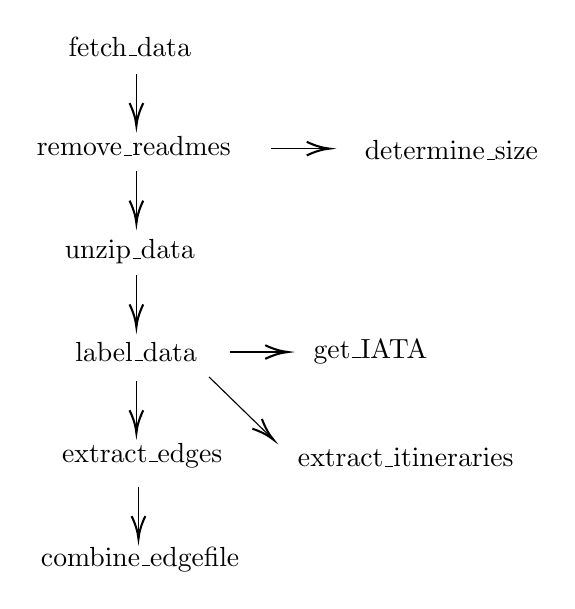
\begin{tikzpicture}[x=0.75pt,y=0.75pt,yscale=-1,xscale=1]
%uncomment if require: \path (0,300); %set diagram left start at 0, and has height of 300

%Straight Lines [id:da774937353877323] 
\draw    (329.2,28.2) -- (329.2,51.2) ;
\draw [shift={(329.2,53.2)}, rotate = 270] [color={rgb, 255:red, 0; green, 0; blue, 0 }  ][line width=0.75]    (10.93,-3.29) .. controls (6.95,-1.4) and (3.31,-0.3) .. (0,0) .. controls (3.31,0.3) and (6.95,1.4) .. (10.93,3.29)   ;

%Straight Lines [id:da37948328121331465] 
\draw    (329.2,75.2) -- (329.2,98.2) ;
\draw [shift={(329.2,100.2)}, rotate = 270] [color={rgb, 255:red, 0; green, 0; blue, 0 }  ][line width=0.75]    (10.93,-3.29) .. controls (6.95,-1.4) and (3.31,-0.3) .. (0,0) .. controls (3.31,0.3) and (6.95,1.4) .. (10.93,3.29)   ;

%Straight Lines [id:da2604231609644325] 
\draw    (394.2,64.2) -- (420.2,64.2) ;
\draw [shift={(422.2,64.2)}, rotate = 180] [color={rgb, 255:red, 0; green, 0; blue, 0 }  ][line width=0.75]    (10.93,-3.29) .. controls (6.95,-1.4) and (3.31,-0.3) .. (0,0) .. controls (3.31,0.3) and (6.95,1.4) .. (10.93,3.29)   ;

%Straight Lines [id:da5664873603541694] 
\draw    (329.2,125.2) -- (329.2,148.2) ;
\draw [shift={(329.2,150.2)}, rotate = 270] [color={rgb, 255:red, 0; green, 0; blue, 0 }  ][line width=0.75]    (10.93,-3.29) .. controls (6.95,-1.4) and (3.31,-0.3) .. (0,0) .. controls (3.31,0.3) and (6.95,1.4) .. (10.93,3.29)   ;

%Straight Lines [id:da979436082222915] 
\draw    (374.2,162.2) -- (400.2,162.2) ;
\draw [shift={(402.2,162.2)}, rotate = 180] [color={rgb, 255:red, 0; green, 0; blue, 0 }  ][line width=0.75]    (10.93,-3.29) .. controls (6.95,-1.4) and (3.31,-0.3) .. (0,0) .. controls (3.31,0.3) and (6.95,1.4) .. (10.93,3.29)   ;

%Straight Lines [id:da2369337782591805] 
\draw    (329.2,176.2) -- (329.2,199.2) ;
\draw [shift={(329.2,201.2)}, rotate = 270] [color={rgb, 255:red, 0; green, 0; blue, 0 }  ][line width=0.75]    (10.93,-3.29) .. controls (6.95,-1.4) and (3.31,-0.3) .. (0,0) .. controls (3.31,0.3) and (6.95,1.4) .. (10.93,3.29)   ;

%Straight Lines [id:da5287233692241446] 
\draw    (330.2,227.2) -- (330.2,250.2) ;
\draw [shift={(330.2,252.2)}, rotate = 270] [color={rgb, 255:red, 0; green, 0; blue, 0 }  ][line width=0.75]    (10.93,-3.29) .. controls (6.95,-1.4) and (3.31,-0.3) .. (0,0) .. controls (3.31,0.3) and (6.95,1.4) .. (10.93,3.29)   ;

%Straight Lines [id:da33374672983323517] 
\draw    (364.2,174.2) -- (393.77,203) ;
\draw [shift={(395.2,204.4)}, rotate = 224.25] [color={rgb, 255:red, 0; green, 0; blue, 0 }  ][line width=0.75]    (10.93,-3.29) .. controls (6.95,-1.4) and (3.31,-0.3) .. (0,0) .. controls (3.31,0.3) and (6.95,1.4) .. (10.93,3.29)   ;


% Text Node
\draw (326,15) node  [align=left] {fetch\_data};
% Text Node
\draw (328,63) node  [align=left] {remove\_readmes};
% Text Node
\draw (481,65) node  [align=left] {determine\_size};
% Text Node
\draw (326,114) node  [align=left] {unzip\_data};
% Text Node
\draw (329,162) node  [align=left] {label\_data};
% Text Node
\draw (442,162) node  [align=left] {get\_IATA};
% Text Node
\draw (332,212) node  [align=left] {extract\_edges};
% Text Node
\draw (331,262) node  [align=left] {combine\_edgefile};
% Text Node
\draw (459,213) node  [align=left] {extract\_itineraries};


\end{tikzpicture}
%     \caption{Operations graph implemented in \texttt{signac-flow}.}
%     \label{fig:operations}
% \end{figure}

Because there are over 100 quarters of data, we needed an organizational scheme that would offer the flexibility to rapidly experiment on one quarter while also scaling to the full data set. To do this, we use the open-source \texttt{signac} framework\footnote{\url{https://signac.io}}. The project workflow script performs operations on each quarter of data using a directed graph of tasks with pre- and post-conditions. The entire operations workflow (from downloading raw data through processing with PySpark) runs on each quarter of data, and each operation can run in series or parallel depending on memory requirements.

We prototyped operations interactively in Jupyter notebooks, configured to interface with the Spark cluster in a real-time session, and then ported into the \texttt{signac-flow} project workflow script. Smaller pre- and post-processing tasks utilized \texttt{pandas}. We ran all job operations (\texttt{bash}, Python, \texttt{pandas}, PySpark) using \texttt{signac-flow}. The entire workflow (downloading input data, parsing and pre-processing, Spark submission, and analysis) can be reproduced or re-run by calling one terminal command.

% =====
% METHODS
% =====
\section{Methods} \label{sec:methods}
% Introduce the method you propose, give the necessary definitions, and potentially give proof of concept.

All code used to run the analysis found in this paper can be found in our GitHub repository: \\ \url{https://github.com/bdice/advanced-data-mining-project}

\subsection{Build first order network from coupon data}
We built directed first-order networks from the coupon trajectories compiled from the raw data as outlined in Section \ref{sec:data}, and weighted the edges by the number of coupons. As a note, we could also weight by the total number of \textit{passengers} on each edge, but since most (>75\%) of coupons are only one passenger, we decided this was an incremental update we did not need.

\subsection{Build a higher-order network (HON) from compiled trajectory data}
First, we merged coupons by their itinerary's unique identifier to form trajectories. We can think of these as trajectories between ``physical nodes,'' i.e. airports.  These trajectories are the input for the \texttt{BuildHON+} algorithm. Previous work on DB1B data by Rosvall et al. made some assumptions about paths' endpoints (e.g. choice of memory nodes) that make the problem simpler and capture helpful dynamics \cite{Rosvall2014}. Specifically, the first and last airports on a ticket are included twice to enforce the inclusion of self-memory nodes that reinforce the importance of a home city over transfer traffic. 

Next, we use a HON-generating algorithm that produces a network of variable-order ``state nodes'' by proposing transition rules. Here, we use the \texttt{BuildHON+} algorithm of Xu et al. \cite{Xu2017}. There is an open-source Python implementation\footnote{\url{https://github.com/xyjprc/hon}} that we adapted for our analysis by reformatting our output to match the package's required structure\cite{Xu2016,Xu2017}.

We allowed the algorithm to dynamically choose its own cutoff order $k$ for each trajectory history by setting a large maximum value ($k = 99$). The algorithm's time complexity is not strongly dependent on $k$ after a certain point, as seen in Table 1 of the HON paper where the run time of $k = 3$ and $k = 5$ differ by only 8\% \cite{Xu2016}. As the average trajectory length is approximately 2.5 legs, it is unlikely that we would even need to worry about such high orders across most of the network. The authors posited that their algorithm's scalability is because there are typically far fewer correlations of high order than low order. Our data seems to agree: over 99.95\% of the edges' weights are between nodes with 4 or fewer orders of history, 93\% with 3 or fewer, and about 66\% with 2 or fewer.

\subsection{Detect communities on the HON using InfoMap}
InfoMap is a community detection algorithm that models a random walker process (MapEquation) on the HON's state nodes (a ``memory network'')\cite{Rosvall2009}. A random walker tends to stay within a community; using the InfoMap algorithm (which minimizes a ``map equation.'' which we'll not cover in further detail here) can be used as a proxy for calculating the real flow through the network. We've leveraged an available implementation in \texttt{C++} and Python\footnote{\url{https://github.com/mapequation/infomap}}, which only required manipulating our input/output file formats.

For visualization, we then merge state nodes (e.g. ``LGA|ORD'') back to physical nodes (``LGA''). InfoMap outputs the proportion of random walks through each state node, which we then use to calculate the ``flow'' through each physical node. This will be referred to repeatedly in Section \ref{sec:experiments}.

One consistent question throughout this semester is how we would measure the ``quality'' of the communities created by InfoMap. We had initially planned to compare ``accuracy'' relative to the communities identified by Rosvall et al. \cite{Rosvall2014}, but that work did not have explicit information about the airport-to-community mappings. We then planned to compare the relative ``performance'' of different community detection methods, e.g. motif-detection community detection algorithm \cite{Benson2016}. Ultimately, we decided to focus on \textbf{verifying that the communities identified via InfoMap were interpretable}, in part due to peer feedback during the Midterm presentations. On this metric, we have been very successful.

% =====
% EXPERIMENTS
% =====
\section{Results} \label{sec:experiments}
% Give some preliminary experiments (on synthetic or real data).
Our implicit hypothesis, unless otherwise stated, is that we will be able to generate findings that are explainable by cross-referencing with common-sense analyses of airline data.

\subsection{First-order network formation validated by known baselines}

\begin{figure}
    \centering
    \includegraphics[width=0.5\textwidth]{figs/PageRank_fon_map.png}
    \includegraphics[width=0.4\textwidth]{figs/PageRank_v_flow.png}
    \caption{(Top) Nodes identified from the data set over period Q1 2011. Node size corresponds to flow through the node while color corresponds to the node's PageRank value based on a first order network, i.e. one that does not take higher-order dependencies into account. (Bottom) For nodes in the largest community in the network, flow is plotted versus PageRank to demonstrate correlation.} 
    \label{fig:fon_pagerank}
\end{figure}

Throughout this project, we were faced with the challenge that we do not have a ``standard of truth'' baseline to compare to. Instead, we have sought to validate our findings by comparing to known trends in the data, beginning with the first order network.

In Figure \ref{fig:fon_pagerank}, we show all nodes (airports, indicated by their IATA code) in the data set with node sizes indicating coupon volume and colors indicating PageRank. We have two checks. First, we would expect that, for a first order network, coupon volume (i.e. the number of coupon ``edges'' including the airport, which we approximate using InfoMap flow) and the PageRank would be correlated. Without higher-order dependencies accounted for, we expect that an airport with many possible edges into it is also one that a random route is more likely to be able to reach (an approximation for PageRank). Indeed, we see these two values are correlated.

Our second check is a gut check. Large nodes with high PageRank should be those airports we would typically consider hubs. Indeed, we find that the top 30 busiest U.S.-based airports by passenger volume in 2017 are all clearly visible on this map, with the exception of Honolulu (HNL, not shown on our continental U.S. representation).\footnote{List of the top 30 airports by passenger volume is not reproduced here, but is readily available on \url{https://en.wikipedia.org/wiki/List_of_the_busiest_airports_in_the_United_States}.}  

\begin{figure}
    \centering
    \includegraphics[width=0.5\textwidth]{figs/seasonality_map.png}
    \caption{Shown above is seasonality of U.S. airports, as measured by PageRank in the first order network. Node colors correspond to the PageRank seasonality correlation coefficient described in the text and indicated on the colorbar. Node sizes correspond to PageRank in 2018 Q3, and labels indicate three letter IATA airport codes.}
    \label{fig:seasonality}
\end{figure}

As we will show shortly, clustering reveals very little information about this first order network. However, we were intrigued to see whether we could find temporal (rather than purely structural) patterns in the data. One obvious temporal pattern is seasonality. We can think of seasonality as ``is this node more `important' to the network in the winter (Q1) or summer (Q3)?'' \footnote{One can think of other temporal patterns: dying cities, airline mergers. We will explore the latter in a following section.}

We calculate the seasonality measure as a time series correlation coefficient over the full set of data. First, the time series of node PageRanks was collected from 1993 Q1 to 2018 Q3. The time series was normalized by subtracting its linear trend and scaling to zero mean and unit variance. The correlation coefficient was computed between this normalized time series and a sinusoidal wave with a one year period with its peak in Q3 and valley in Q1. In Figure \ref{fig:seasonality}, we show nodes colored by this correlation coefficient measuring their PageRank seasonality.

Figure \ref{fig:seasonality} provides more trend-analysis evidence validation of our network structures. We see that the south-- particularly Florida and the desert Southwest-- has strong winter seasonality, explained by vacation and retiree travel. Further, we see a trail of blue through the Rocky Mountains, corresponding to the winter ski season. The inverse, strong summer activity, is less stark. However, strong summer seasonality of Portland and Seattle corresponds to the few non-grey months of the year and the peak of the Pacific Northwest tourist season.

\subsection{HONs accurately account for regional airline communities.}
\begin{figure*}
    \centering
    \includegraphics[width=\textwidth]{figs/FON_vs_HON.png}
    \caption{Shown are the communities identified using InfoMap for (a) a first order network and (b) a higher-order network. Only one community (the largest) is shown for the first order network, while the 5 largest communities are shown for the HON. Data is a snapshot from 2011 Q1. Node colors indicate communities, and sizes correspond to flow volume, defined in the text. Labels indicate three letter IATA airport codes.}
    \label{fig:fon-vs-hon}
\end{figure*}

Our hypothesis when making HONs from the flight coupon data was that community detection would yield more ``meaningful'' communities on a HON versus a first order network. While we did not have a clear metric for what this would entail, the results were strikingly different betweent the two methods. In Figure \ref{fig:fon-vs-hon}, we show the largest community identified using InfoMap for (a) a first order network and (b) the five largest communities, colored uniquely, identified on a HON.

In the first order network, a single massive community encompassing flights within the continental United States and Hawaii accounts for 99.7\% of all flight data. The next two largest communities are the much smaller sets of flights between Alaska and the continental United States, and flights within Alaska. Neither is shown, given their small numbers. We will stick with the continental U.S. representation from here on out.

For a higher-order network, we see that the communities are much more selective. As such, we would expect that each holds more information about its population. We observe that each individual community is typically a regional collection of small airports and a few of their regional hubs. However, we were hoping to move beyond the shipping network example given earlier and identify deeper insights from the data. To do this, we zoom in on the largest community identified in Figure \ref{fig:fon-vs-hon}b.

\subsection{HON communities identified using community detection correspond to real-world networks}
\begin{figure*}
    \centering
    \includegraphics[width=\textwidth]{figs/example_community.png}
    \caption{Shown is the largest community identified using InfoMap from 2011 Q1 (top) and a select community from 2013 Q1 (bottom). At left (a/c), we highlight the primary nodes present in each community. Map node color and size indicates PageRank (see colorbar). Labels indicate three letter IATA airport codes. At right (b/d), the distribution of carriers as a percentage of flow through the community is shown by two-letter call sign.
    }
    \label{fig:community}
\end{figure*}
We highlight the largest community from Figure \ref{fig:fon-vs-hon}b (colored in blue) in Figure \ref{fig:community}a. Here, we color nodes by their PageRank. In the inset, we observe that the largest nodes in the community are PIT (Pittsburgh), PHL (Philadelphia), CLT (Charlotte), and to smaller extents DCA (Washington, D.C.) and BOS (Boston). To an informed observer, these hubs suggest that this community largely encompasses US Airways, a now-extinct airline that merged with American Airlines in 2015.

Indeed, a double-click on this data in Figure \ref{fig:community}b reveals that over half the ticket volume in the community is represented by US Airways (US). This real-world interpretation of our data validates that communities found in a HON embed deeper information than the structurally-simpler first-order network can contain.

Previously, we had planned to compare our results to those identified by Rosvall et al. \cite{Rosvall2014}. Unfortunately, that paper doesn't contain actual examples of communities given by community detection on an order-2 HON; it instead focuses much more on the impact of a HON representation on the quality of ``memory'' that was contained. Our HON is, on average, of order $2.394$ in the edge destinations and order $1.819$ in the edge sources; comparing our variable $k$-order networks with a strictly second-order network would be an interesting follow-on work.

However, one could argue that the above sample is a biased representation of the quality of community found using InfoMap on a HON of the flight data, as US Airways was the largest airline by ticket volume in 2011. As a counter-example, we highlight a community containing the Seattle (SEA) and Portland (PDX) airports in Figure \ref{fig:community}c and d. Here, we see that the ticket volume is dominated by AS-- Alaska Airlines. While Alaska Airlines is a major player in the U.S. airline market, it was only the seventh-largest by passenger volume in 2011.\footnote{\url{https://en.wikipedia.org/wiki/List_of_largest_airlines_in_North_America}} Many of its routes are in or out of the Pacific Northwest, and it is headquartered in Seattle.

\subsection{HON community detection highlights airline mergers and reveals preserved underlying route structure, even after integration is completed}

\begin{figure*}
    \centering
    \includegraphics[width=\textwidth]{figs/DL_NW_merger.png}
    \caption{Shown are data for (a) 2004 Q3 and (b) 2013 Q1. Delta (DL) and Northwest (NW) officially merged in 2010 Q1. Interestingly, we observe that this merger did not lead to major structural changes in the networks. Community numbers in the headers correspond to the order in which they were found by the InfoMap algorithm, and are not otherwise meaningful. For each community, the associated pie chart indicates the carriers represented, weighted by flow through the community. In the maps, node color and size indicates flow in the community (see colorbar). Labels indicate three letter IATA airport codes.}
    \label{fig:merger}
\end{figure*}

The observation that US Airways dominated the largest community in 2011 but is no longer an independent airline raised an interesting question for us: could we use community detection to observe the role of mergers in the structure of airline traffic data in the U.S.? Na\"ively, we might expect that mergers will combine multiple independent communities into larger, aggregated ones.

This is of particularly interest as the late 2000s and early 2010s saw a number of large airline mergers, e.g. US Airways/American (2015 Q2), Northwest/Delta (2010 Q1), and Continental/United (2011 Q4). As DTW is our local airport, and now a Delta hub, we zoomed in on the Northwest/Delta merger.

At least at the large community level, our hypothesis that ``one community to rule them all'' would emerge proved incorrect. Interestingly, we see that the underlying structure in the flight tickets is preserved. In Figure \ref{fig:merger}a, we see snapshots of the largest Delta (DL, left) and Northwest (NW, right) communities in 2004 Q1. Delta is based in Atlanta (ATL) and used it and Cincinnati (CVG) as its major hubs. Northwest, at that time, was the major player in the Midwest, with hubs in Minneapolis (MSP) and Detroit (DTW).

We take another snapshot in 2013 Q1, three years after the merger is complete (Figure \ref{fig:merger}b). Instead of seeing one major combined Delta community, we see two largely non-overlapping ones. Fascinatingly, this suggests that airline mergers do not significantly change the underlying transportation network structure. This same pattern holds for investigations of the US Airways/American and Continental/United mergers. Indeed, this indicates that mergers and their accompanying ticket name changes are merely business branding decisions, rather than structural network shifts. The only notable change we see between pre/post-merger for the Delta network is the increased flow through Atlanta from the old Northwest network. This indicates that some additional inter-community flow has been added, but not in a structurally significant way.

There is some chance that great structural changes would be seen for smaller communities. However, at that point we will be looking at individual nodes and their connecting airports; this is unlikely to be practically meaningful.


% ======
% RELATED WORK
% ======
\section{Related work}
% discuss the shortcomings of these papers

\subsection{Structural analysis of transportation data}

Past work on the DB1B airline itinerary data set has used a fixed second-order network on data from 2011 Q1 to Q3 \cite{Rosvall2014}. This data set was a benchmark for their HON model which shows much less entropy in the MapEquation model for a second-order network compared to a first-order network. This study found that 79\% of the paths in the data were of length 3 or greater, though the network used for analysis was strictly second order. 

Variable higher-order networks coupled with community detection, have also been been used for analyzing shipping transportation data \cite{Xu2016, Xu2017}. These papers introduced the \texttt{BuildHON+} algorithm we utilized in this work, and demonstrated that community detection on HONs yielded structural insights missing from first order representations. Xu et al. also utilize InfoMap to build communities from their data; for that reason (as well as those discussed previously in the text) we use that same method here\cite{Rosvall2014}.

\subsection{Methods for forming higher-order networks from trajectory data}

There are two primary ways to form higher-order networks from trajectory-like data. The simplest approach is to take a fixed order $k$ and divide each of the graph's $N$ physical nodes into ``state nodes'' representing trajectories of length $k$ ending with that physical node. These state nodes encode the history of a trajectory, e.g. $\vec{hij}$ might represent a state node for the physical node $j$ which had previously visited $h$ and $i$ before arriving at $j$ \cite{Rosvall2014}. Fixed order representations must ignore trajectories with total length less than $k$, since the trajectory cannot be represented in a second order state node \cite{Rosvall2014}. Additionally, the number of state nodes must increase as $N^k$ to record all possible trajectories, limiting this approach to small $k$ (typically 2) \cite{Rosvall2014}. A more complex representation is that of Xu et al. \cite{Xu2016}, later improved to be parameter-free \cite{Xu2017}, where the order is determined dynamically from data: state nodes represent trajectories of variable length, and higher-order state nodes are created if and only if their creation is statistically significant for the network's predictive power. This method allows for a sparse representation that can capture higher-order dynamics than fixed-order models, which are computationally constrained by the explosive growth in state nodes as $k$ increases. As the authors clarify, ``if the dependency is assumed as fixed second order, it could be redundant when first-order dependencies are sufficient and could be insufficient when higher-order dependencies exist'' \cite{Xu2016}.

\subsection{Community detection, clustering, and other centrality algorithms for higher-order networks} 

An insight of Xu et al. is that typical network analysis methods, such as clustering, centrality, and ranking, can be applied to study higher-order networks, once a network of higher-order state nodes has been produced \cite{Xu2016}. For instance, they apply MapEquation, a clustering algorithm based on the entropy of random walks, to a shipping data set. By merging the state nodes into physical nodes at the end, they naturally reveal a rich overlapping community structure, with important implications for studying the transmission of invasive species. This structure is hidden in the first-order network analysis.

\subsection{Workflow management for data analysis}
Other works using the \texttt{signac} data management framework have largely been focused in the domains of materials science and computational physics \cite{signac_commat,Teich2019,Thompson2019}. To our knowledge, this is the first application of the framework to graph mining. Because graph manipulation and computations are often file-based workflows, this is a natural fit for the framework's design.

% ======
% CONCLUSIONS
% ======
\section{Conclusions}
Higher-order networks reveal network structure and dynamics not apparent in a first-order representation. Using community detection on higher-order networks, we found interpretable features of airline networks in the United States. Previous works have focused on either identifying clusters on variable higher-order networks of shipping data \cite{Xu2016}, or community detection on second order networks of flight data among other data sets \cite{Rosvall2014}. 

\textbf{To the best of our knowledge, this is the first example of using a variable $k$-order HON to study flight traffic data and demonstrate that community detection yields interpretable results.}

Additionally, we provide an example of using a Python-based data management framework (\texttt{signac} and \texttt{signac-flow}) for a data-mining project. We hope to build this test case out as a public example of how to use these packages for data mining project management. 

Looking forward, an interesting follow-up we could consider would be comparing the performance of InfoMap versus a more traditional method (e.g. Louvain) in identifying interpretable communities on this network. While the two methods mentioned have already been benchmarked against one another \cite{Rosvall2014}, we would argue that interpretability is the key property needed for analysis of business-facing data. We're pleased that this paper contributes to that point of view.

% ======
% DISTRIBUTION OF WORK
% ======
\section{Distribution of work}
Volume of the work was evenly distributed from the viewpoint of the team. Responsibility biases were approximately as follows: Bradley spearheaded fetching and cleaning data and analysis code development with PySpark; Daniel built HONs and implemented Pythonic InfoMap for community detection; Shannon planned and interpreted analysis and spearheaded writing of the written deliverables (poster, report).

\newpage
\bibliographystyle{ACM-Reference-Format}
\bibliography{midterm}

\end{document}
